\section{Simulator Evaluation}

To ensure that our system meets the quality standards necessary for research purposes and accurately simulates a volumetric display, we conducted a comprehensive evaluation using various metrics.

\subsection{Comparison to Other Systems}

The field of volumetric displays is relatively niche, but there are a few comparable systems available if we expand our criteria to include related fields. Table~\ref{table:comparison} provides a comparison of our system to other systems based on the various features they support. "Single Camera" refers to whether the system can operate with a single camera or requires a multi-camera setup. "Custom Display" indicates whether the system necessitates a custom-made display (not a standard projector/monitor). "Stereo" refers to whether the system supports stereo rendering (differing view per eye), and "Multi-User" specifies whether the system supports multiple users viewing simultaneously. \\

Our system is unique in that, to the best of our knowledge, it is the only system that supports single-camera, glasses-free eye and hand tracking. Almost every other system requires a multi-camera setup and the use of IR tracking points, along with a tool for interacting with the volumetric display, rather than offering direct hand tracking capabilities \cite{913797}. \\

Despite these advancements, our system has certain limitations, such as the lack of multi-user support and stereo rendering. These are areas that could be addressed in future work, potentially through the introduction of polarized or shutter glasses.

\begin{table}[h!]
	\stepcounter{globalFigureCounter}
    \centering
    \resizebox{\textwidth}{!}{
    \begin{tabular}{|c|c|c|c|c|c|c|}
        \hline
        \textbf{System} & \textbf{Single Camera} & \textbf{Hand Tracking} & \textbf{Custom Display} & \textbf{Glasses} & \textbf{Stereo} & \textbf{Multi-User}  \\
        \hline
        Volumetric Simulator (\textbf{ours}) & \textbf{\textcolor{Green}{True}} & \textbf{\textcolor{Green}{True}} & \textbf{\textcolor{Green}{False}} & \textbf{\textcolor{Green}{False}} & \textbf{\textcolor{red}{False}} & \textbf{\textcolor{red}{False}} \\
        \hline
        CoGlobe \cite{10.1145/3214907.3214914} \cite{7892376} \cite{10.1145/3290605.3300763} \cite{10.1145/3281505.3281540} & \textbf{\textcolor{red}{False}} & \textbf{\textcolor{red}{False}} & \textbf{\textcolor{red}{True}} & \textbf{\textcolor{red}{True}} & \textbf{\textcolor{Green}{True}} & \textbf{\textcolor{Green}{True}} \\
        \hline
        OrbeVR \cite{10.1145/3084822.3091104} \cite{article-spheree} & \textbf{\textcolor{red}{False}} & \textbf{\textcolor{red}{False}} & \textbf{\textcolor{red}{True}} & \textbf{\textcolor{red}{True}} & \textbf{\textcolor{Green}{True}} & \textbf{\textcolor{Green}{True}} \\
        \hline
        pCubee \cite{10.1145/1753326.1753535} \cite{article_cubee} & \textbf{\textcolor{orange}{Headtracker}} & \textbf{\textcolor{red}{False}} & \textbf{\textcolor{red}{True}} & \textbf{\textcolor{Green}{False}} & \textbf{\textcolor{red}{False}} & \textbf{\textcolor{red}{False}} \\
        \hline
        HandheldBall \cite{10.1145/3025453.3025806} & \textbf{\textcolor{red}{False}} & \textbf{\textcolor{red}{False}} & \textbf{\textcolor{red}{True}} & \textbf{\textcolor{red}{True}} & \textbf{\textcolor{Green}{True}} & \textbf{\textcolor{Green}{True}} \\
        \hline
        TeleHuman \cite{10.1145/2207676.2208640} & \textbf{\textcolor{red}{False}} & \textbf{\textcolor{red}{False}} & \textbf{\textcolor{red}{True}} & \textbf{\textcolor{Green}{False}} & \textbf{\textcolor{red}{False}} & \textbf{\textcolor{red}{False}} \\
        \hline
        HoloDesk \cite{10.1145/2207676.2208405} & \textbf{\textcolor{red}{False}} & \textbf{\textcolor{Green}{True}} & \textbf{\textcolor{red}{True}} & \textbf{\textcolor{Green}{False}} & \textbf{\textcolor{red}{False}} & \textbf{\textcolor{red}{False}} \\
        \hline 
        FaceTrack \cite{10.1109/3DUI.2008.4476617} & \textbf{\textcolor{Green}{True}} & \textbf{\textcolor{red}{False}} & \textbf{\textcolor{Green}{False}} & \textbf{\textcolor{Green}{False}} & \textbf{\textcolor{red}{False}} & \textbf{\textcolor{red}{False}} \\
        \hline
        3DDisplaySimulation \cite{Zabarauskas2012} & \textbf{\textcolor{Green}{True}} & \textbf{\textcolor{red}{False}} & \textbf{\textcolor{Green}{False}} & \textbf{\textcolor{Green}{False}} & \textbf{\textcolor{red}{False}} & \textbf{\textcolor{red}{False}} \\
        \hline
    \end{tabular}}
    \caption{Comparison of systems based on attributes}
    \label{table:comparison}
\end{table}

\subsection{Tracking System}

To gain deeper insights into the performance and quality of the tracking system, we conducted several tests. The primary focus was on the inter-update gap, defined as the time interval between consecutive tracker frames being sent to the renderer.

\begin{figureBox}[label={fig:framerate-overall}, width=1.0\linewidth]{Tracker Inter-Update Gap (over 5 mins)}
    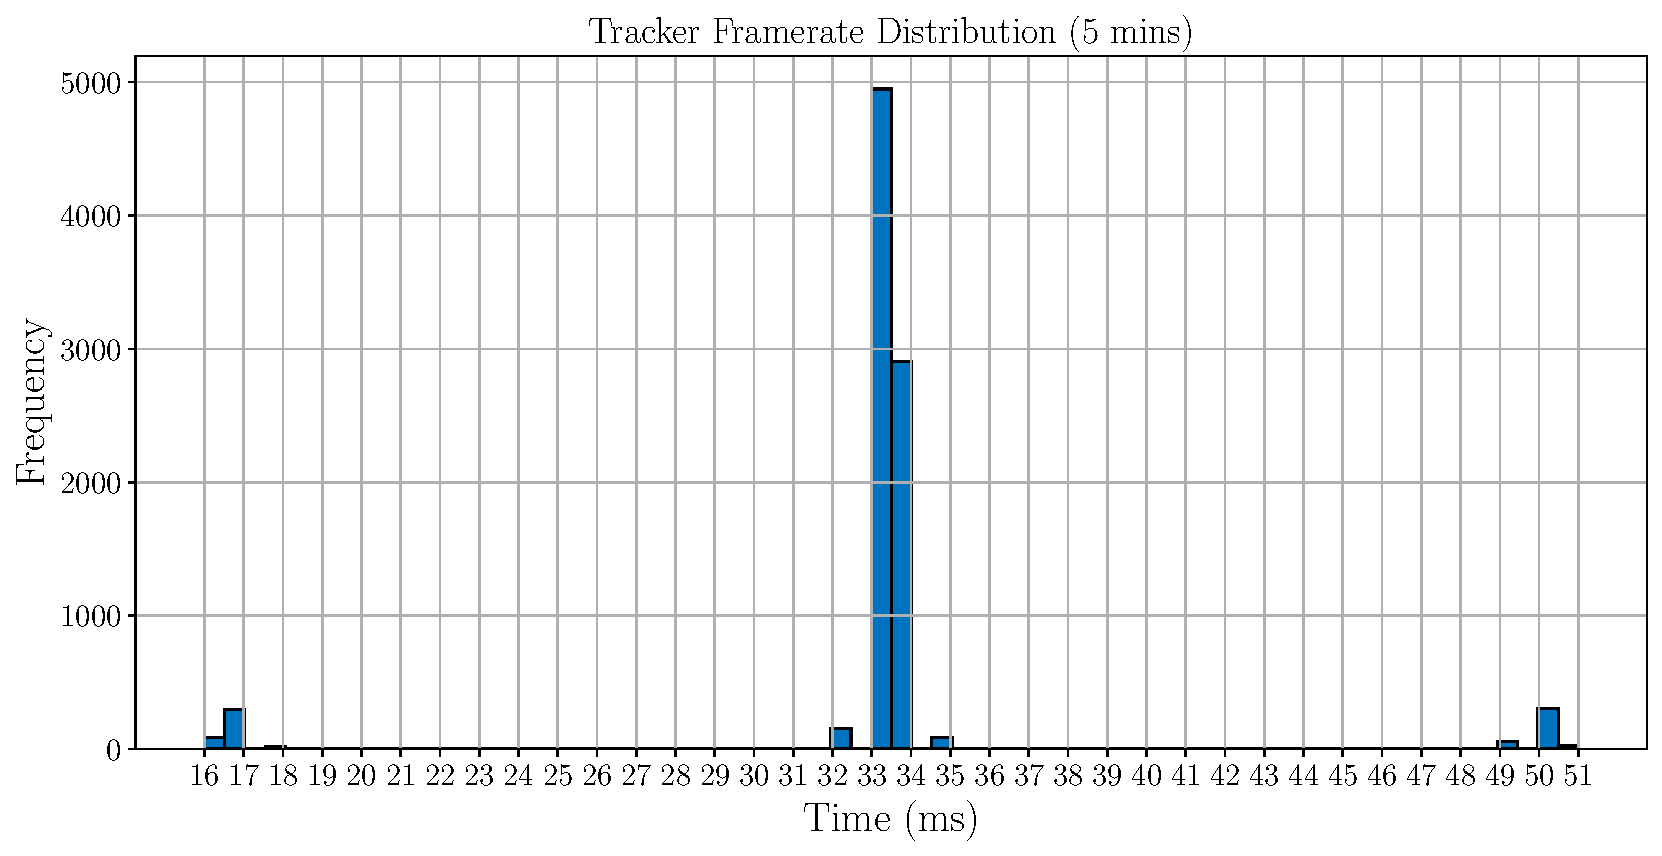
\includegraphics[width = 1.0\linewidth]{./evaluation/figures/framerate-overall.pdf}
\end{figureBox}

As depicted in Figure \ref{fig:framerate-overall}, the system's frame rate remained relatively consistent, with 90.83\% of frames maintaining a latency between 30 and 35 ms. A peculiar observation was the cluster of latencies at 16-18 ms (4.46\%) and 49-51 ms (4.39\%). This anomaly is attributed to the frame rate of the renderer, as our system performs lazy conversion of 2D points to 3D only when necessary. Our renderer operates at 60 fps, constrained by our monitors, resulting in frame intervals approximating to 16.666 ms. Although our tracker functions at 30 fps (33.33 ms inter-update gap), there can be an inter-update gap of 16 ms if the tracker is delayed past the initial 33.33 ms, causing an additional delay of approximately 16.66 ms, resulting in a total gap of around 50 ms. However, during this waiting period, another frame is processed and ready for the next cycle, giving the appearance of a higher frame rate than 30 fps.

\subsubsection{Downscaling Benchmarks}

In exploring the impact of downscaling on performance, we determined that a single instance of downscaling sufficed to meet our performance requirements. Further downscaling did not yield significant performance benefits and adversely affected tracking quality. Figure \ref{fig:pydown} illustrates our findings, showing a noticeable performance improvement when reducing the resolution from the source $2048 \times 1536$ to $1024 \times 793$. Additional reductions in resolution did not provide further speed benefits, as the bottleneck was the 30 fps frame rate of the Kinect camera.

\begin{figureBox}[label={fig:pydown}, width=0.8\linewidth]{Comparing Inter-Update Gap By Resolutions (over 1 min)}
    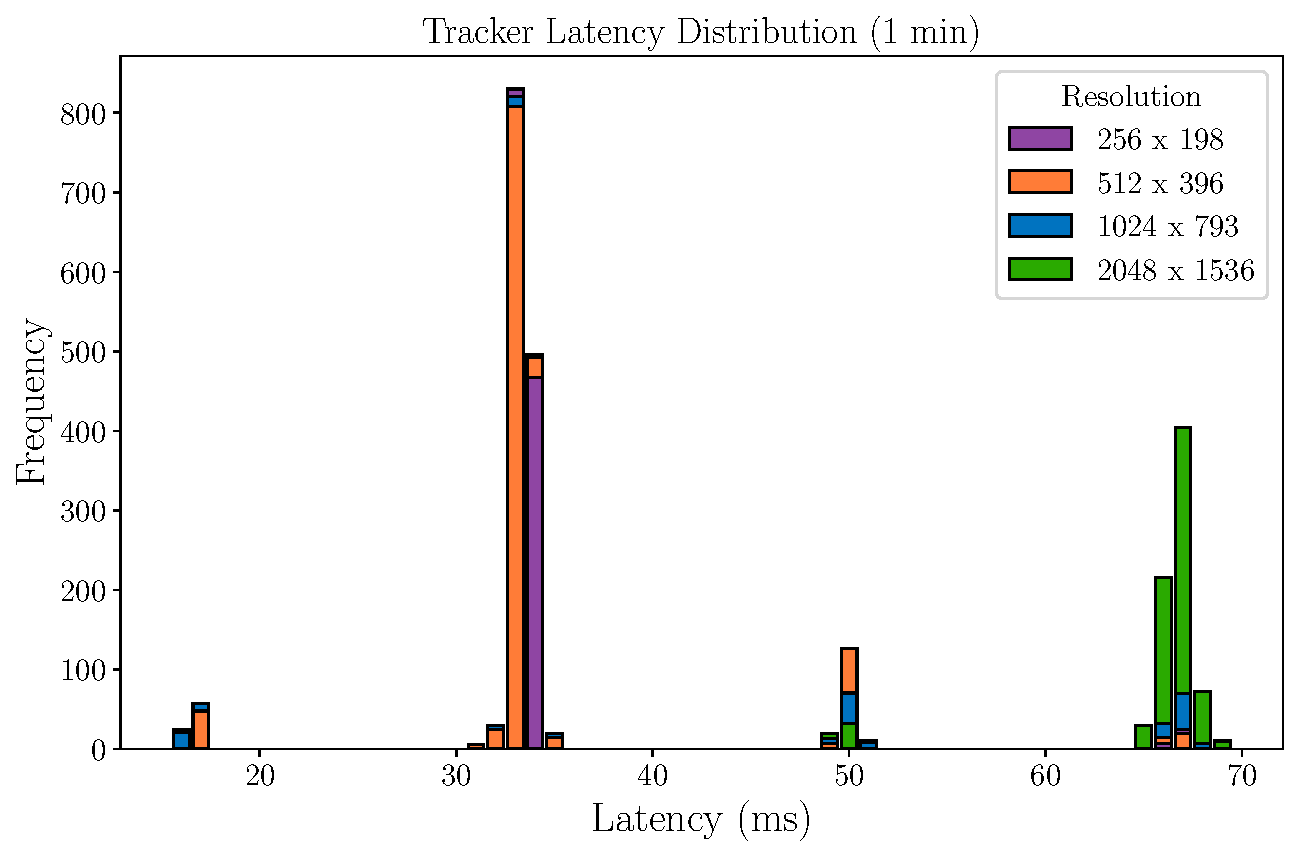
\includegraphics[width = 1.0\linewidth]{./evaluation/figures/pydown.pdf}
\end{figureBox}

\subsubsection{Timings by Subprocess}

Further investigation revealed that among the three concurrent threads (capturing from the Kinect camera, tracking hand and eye movements, and rendering with OpenGL), the primary bottleneck was waiting for the Kinect camera to complete the capture. Figure \ref{fig:process-times-distributions} highlights that expediting the tracking algorithm offered limited benefit due to this bottleneck.

\begin{figureBox}[label={fig:process-times-distributions}, width=0.8\linewidth]{Comparing Thread Competition Times}
    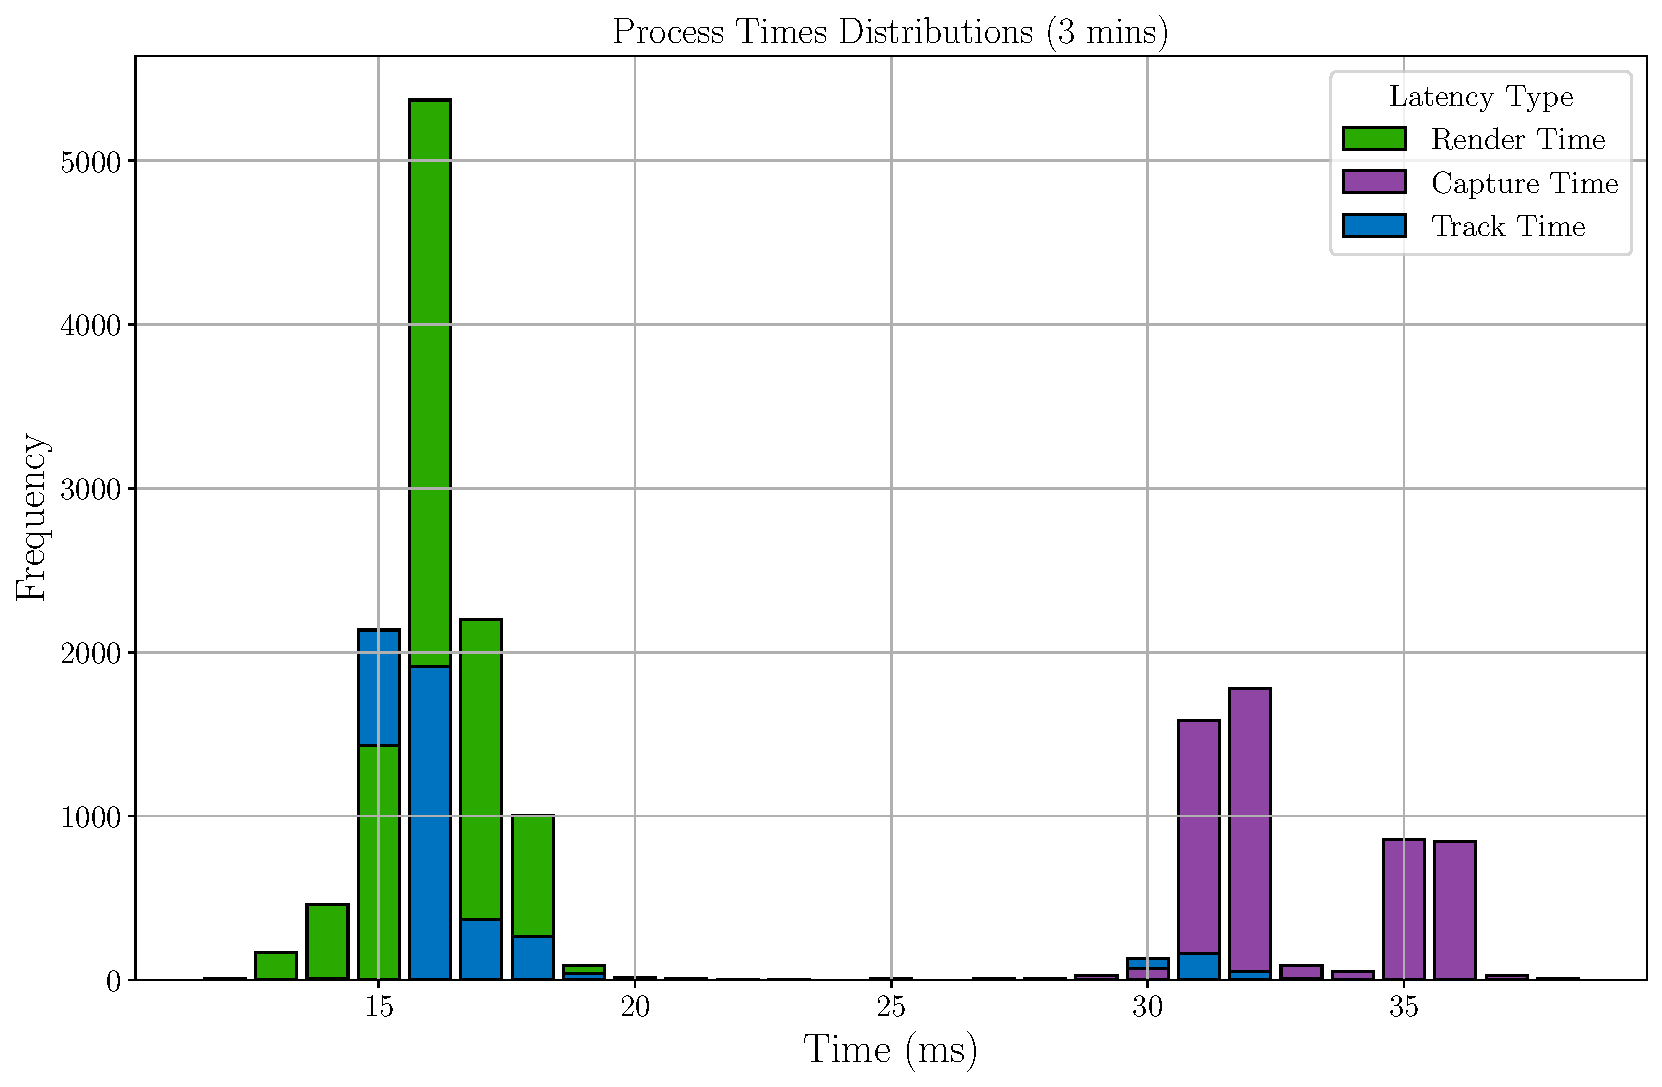
\includegraphics[width = 1.0\linewidth]{./evaluation/figures/process-times-distributions.pdf}
\end{figureBox}

\subsubsection{Latency from Camera to Eye}

Although precise latency statistics for the Azure Kinect from capture to device are unavailable, estimates suggest a latency of around 90 ms \cite{gholami2023autodepthnet}. Considering the time required for OpenGL primitives to display images on the screen, which ranges from 10 to 30 ms depending on the display \cite{https://doi.org/10.1002/jsid.1104} \cite{noauthor_latency_nodate}, and combining this with our system's processing time of less than 30 ms, we estimate the total system latency to be approximately 150 ms. \\

When compared to state-of-the-art systems in similar fields such as VR, our system exhibits higher latency, as shown in Table \ref{tab:photon-to-photon-latency}.

\begin{table}[h!]
	\stepcounter{globalFigureCounter}
    \centering
    \caption{Our Photo-to-Photon Latency Vs Common VR Systems reported by OptoFidelity \cite{noauthor_apple_2024}}
    \label{tab:photon-to-photon-latency}
    \begin{tabular}{lS[table-format=1.2e+2]S[table-format=4.0]S[table-format=2.6]S[table-format=1.6]}
        \toprule
        \textbf{System} & \textbf{Latency (ms)}\\
        \midrule
        \texttt{Volumetric Simulator (\textbf{Ours})} & ~150ms \\
		\texttt{HTC VIVA XR Elite} & ~40ms\\
		\texttt{Meta Quest 3} & ~39ms \\
		\texttt{Meta Quest Pro} & ~38ms \\
        \texttt{Apple Vision Pro} & ~11ms  \\
        \bottomrule
    \end{tabular}
\end{table}

It is challenging to directly compare our system with other similar systems, such as the Multi-person Fish-Tank Virtual Reality Display \cite{10.1145/3281505.3281540} \cite{10.1145/169059.169066} or systems used in 3D Display Simulation Using Head-Tracking with Microsoft Kinect \cite{Zabarauskas2012}, as they do not report their latencies. However, given that both systems utilize Kinect cameras, which are a significant source of latency, we can infer that our system likely has comparable latency to these systems.

\subsubsection{Effective Range}

\begin{invisBox}
    \pictureBox[label={fig:distance-setup}]{Setup for Distance Testing}{
        \adjustbox{height=5cm, keepaspectratio}{
            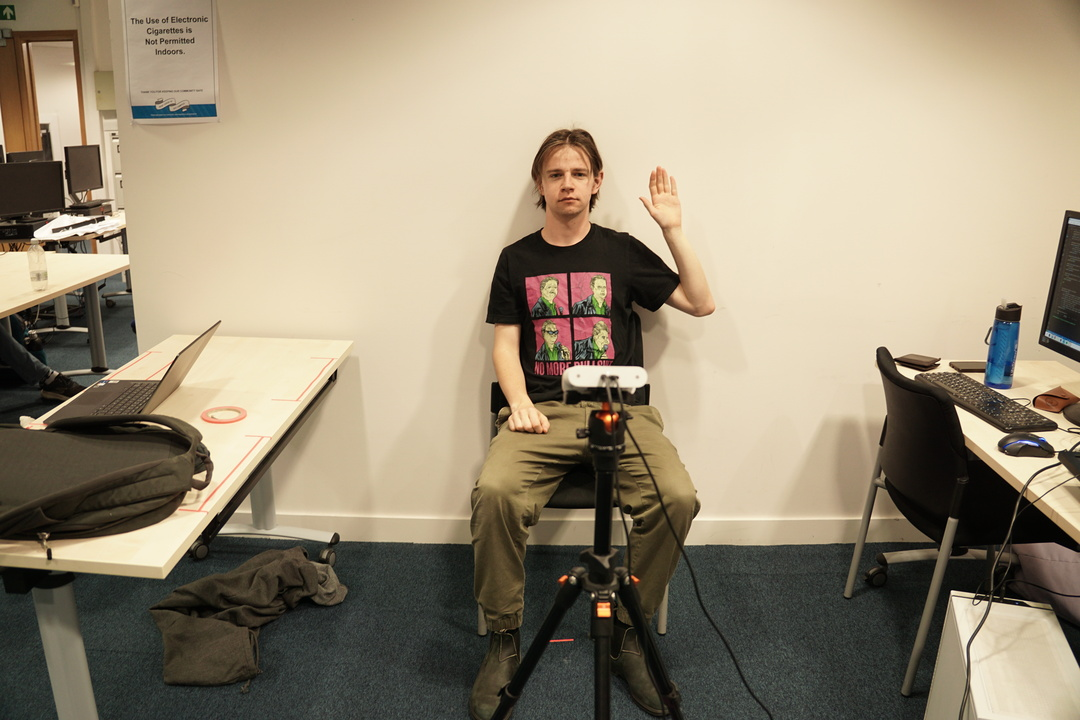
\includegraphics{./evaluation/figures/distance_setup.jpg}
        }
    }
    \hfill
    \pictureBox[label={fig:track-distance}]{Success Rate at Varying Distances}{
        \adjustbox{height=5.0cm, keepaspectratio}{
            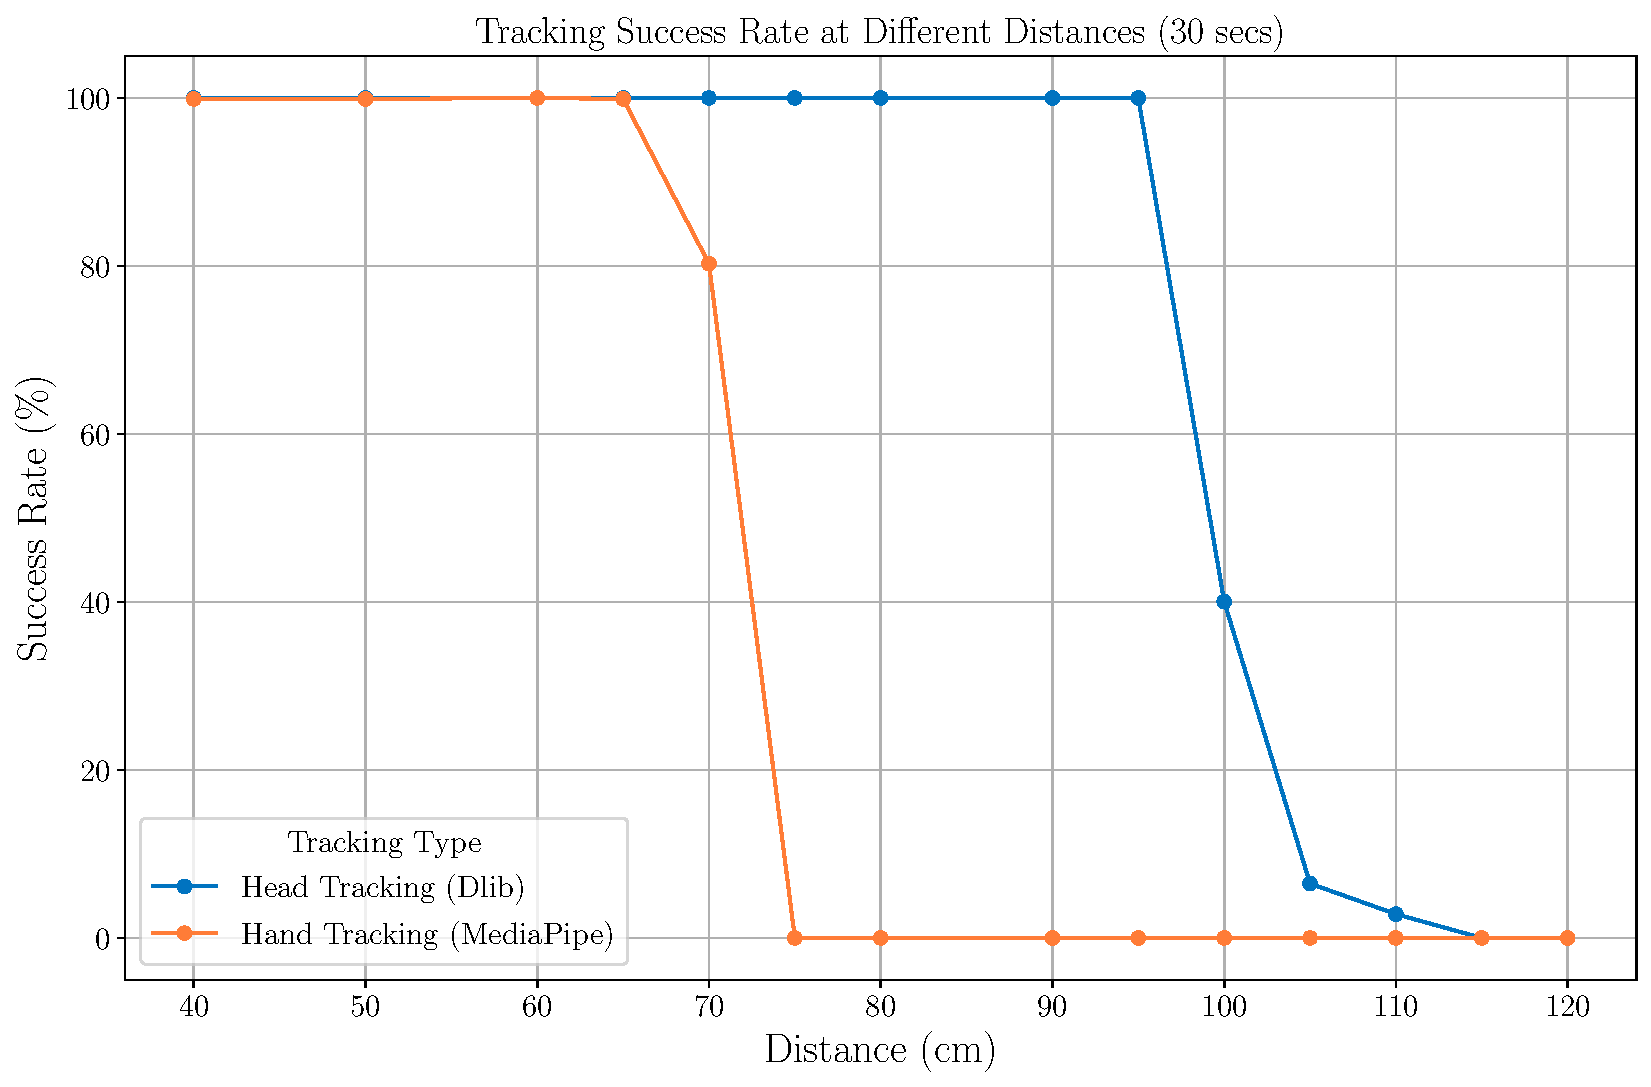
\includegraphics{./evaluation/figures/tracking-success-rate.pdf}
        }
    }
\end{invisBox}


For another important aspect of our evaluation we focused on investigating the effective tracking range of our system. We placed a participant in a fixed position on a chair and instructed them to slowly wave their hand and move their head. An example of the test setup is shown in Figure~\ref{fig:distance-setup}. We conducted tests at various distances, recording the percentage of successful captures that detected a face or hand at 30-second intervals. The resolution of the color image used for this test was $1024 \times 793$.

As illustrated in Figure~\ref{fig:track-distance}, the success rate for MediaPipe's hand tracking model rapidly decreases after 1 meter, ultimately failing 100\% of the time at greater distances. This is likely due to the dataset it was trained on and its primary design for tracking hands using a mobile phone camera \cite{dlib09}. \\

Dlib's head tracking model performed better, with effective tracking up to approximately 1.5 meters. The decline in performance beyond this distance is similarly attributed to the nature of its training data. These findings were considered in the design of our user study, where the camera was positioned to keep the user's hand within 30-70 cm and the head within 1 meter from the camera.

\subsubsection{Head Tracking}

The effectiveness of the head tracking system is another critical aspect, particularly the range of head positions at which tracking is possible. Specifically, we were interested in the angle at which the model fails to detect a face. We set up a straightforward experiment, shown in Figure~\ref{fig:angle-setup}, to measure the head angles at which the tracking system ceases to function. Participants were seated on a swivel chair and asked to keep their body still while rotating their head. We noted the position of the midpoint of their feet when tracking failed, and used basic trigonometry to estimate the head angle.

\begin{figureBox}[label={fig:angle-setup}, width=1.0\linewidth]{Angle Setup}
    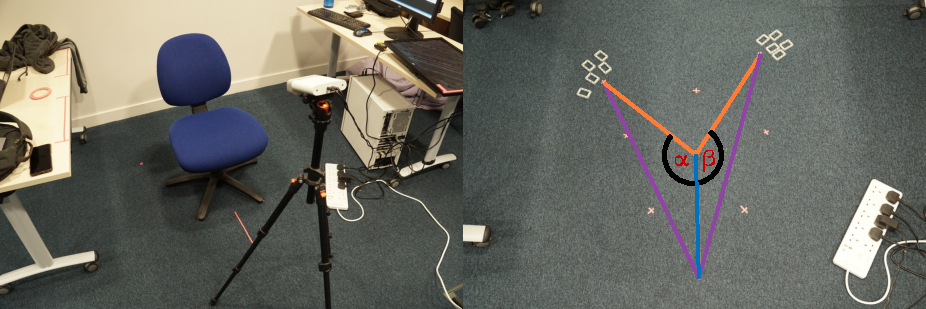
\includegraphics[width = 1.0\linewidth]{./evaluation/figures/angle-setup.pdf}
\end{figureBox}

This test involved five participants, with results presented in Figure~\ref{fig:head-angle}. Although the technique was somewhat rudimentary and thus not highly precise, the angle at which head tracking typically failed ranged between $120^{\circ}$ and $150^{\circ}$. This result may seem counterintuitive, as at these angles, the participant is facing away from the camera. However, the face tracking model first detects a face and then maps landmarks to it, even when the face is not directly visible.

\begin{invisBox}
    \pictureBox[label={fig:head-angle}]{Angle of Failure for Head Tracking}{
        \adjustbox{height=6cm, keepaspectratio}{
            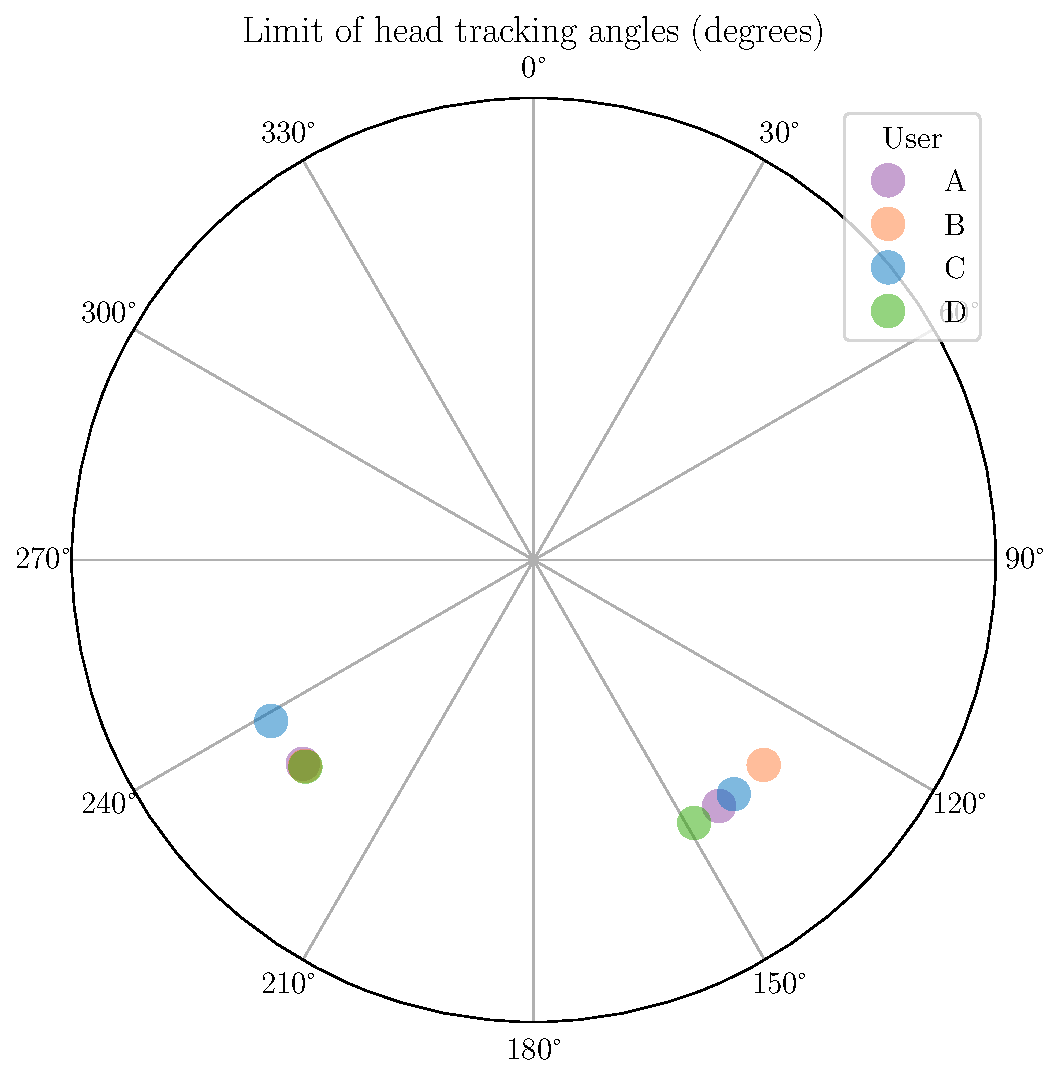
\includegraphics{./evaluation/figures/user-angles.pdf}
        }
    }
    \hfill
    \pictureBox[label={fig:incorrect-head-track}]{Incorrect Head Tracking}{
        \adjustbox{height=6.5cm, keepaspectratio}{
            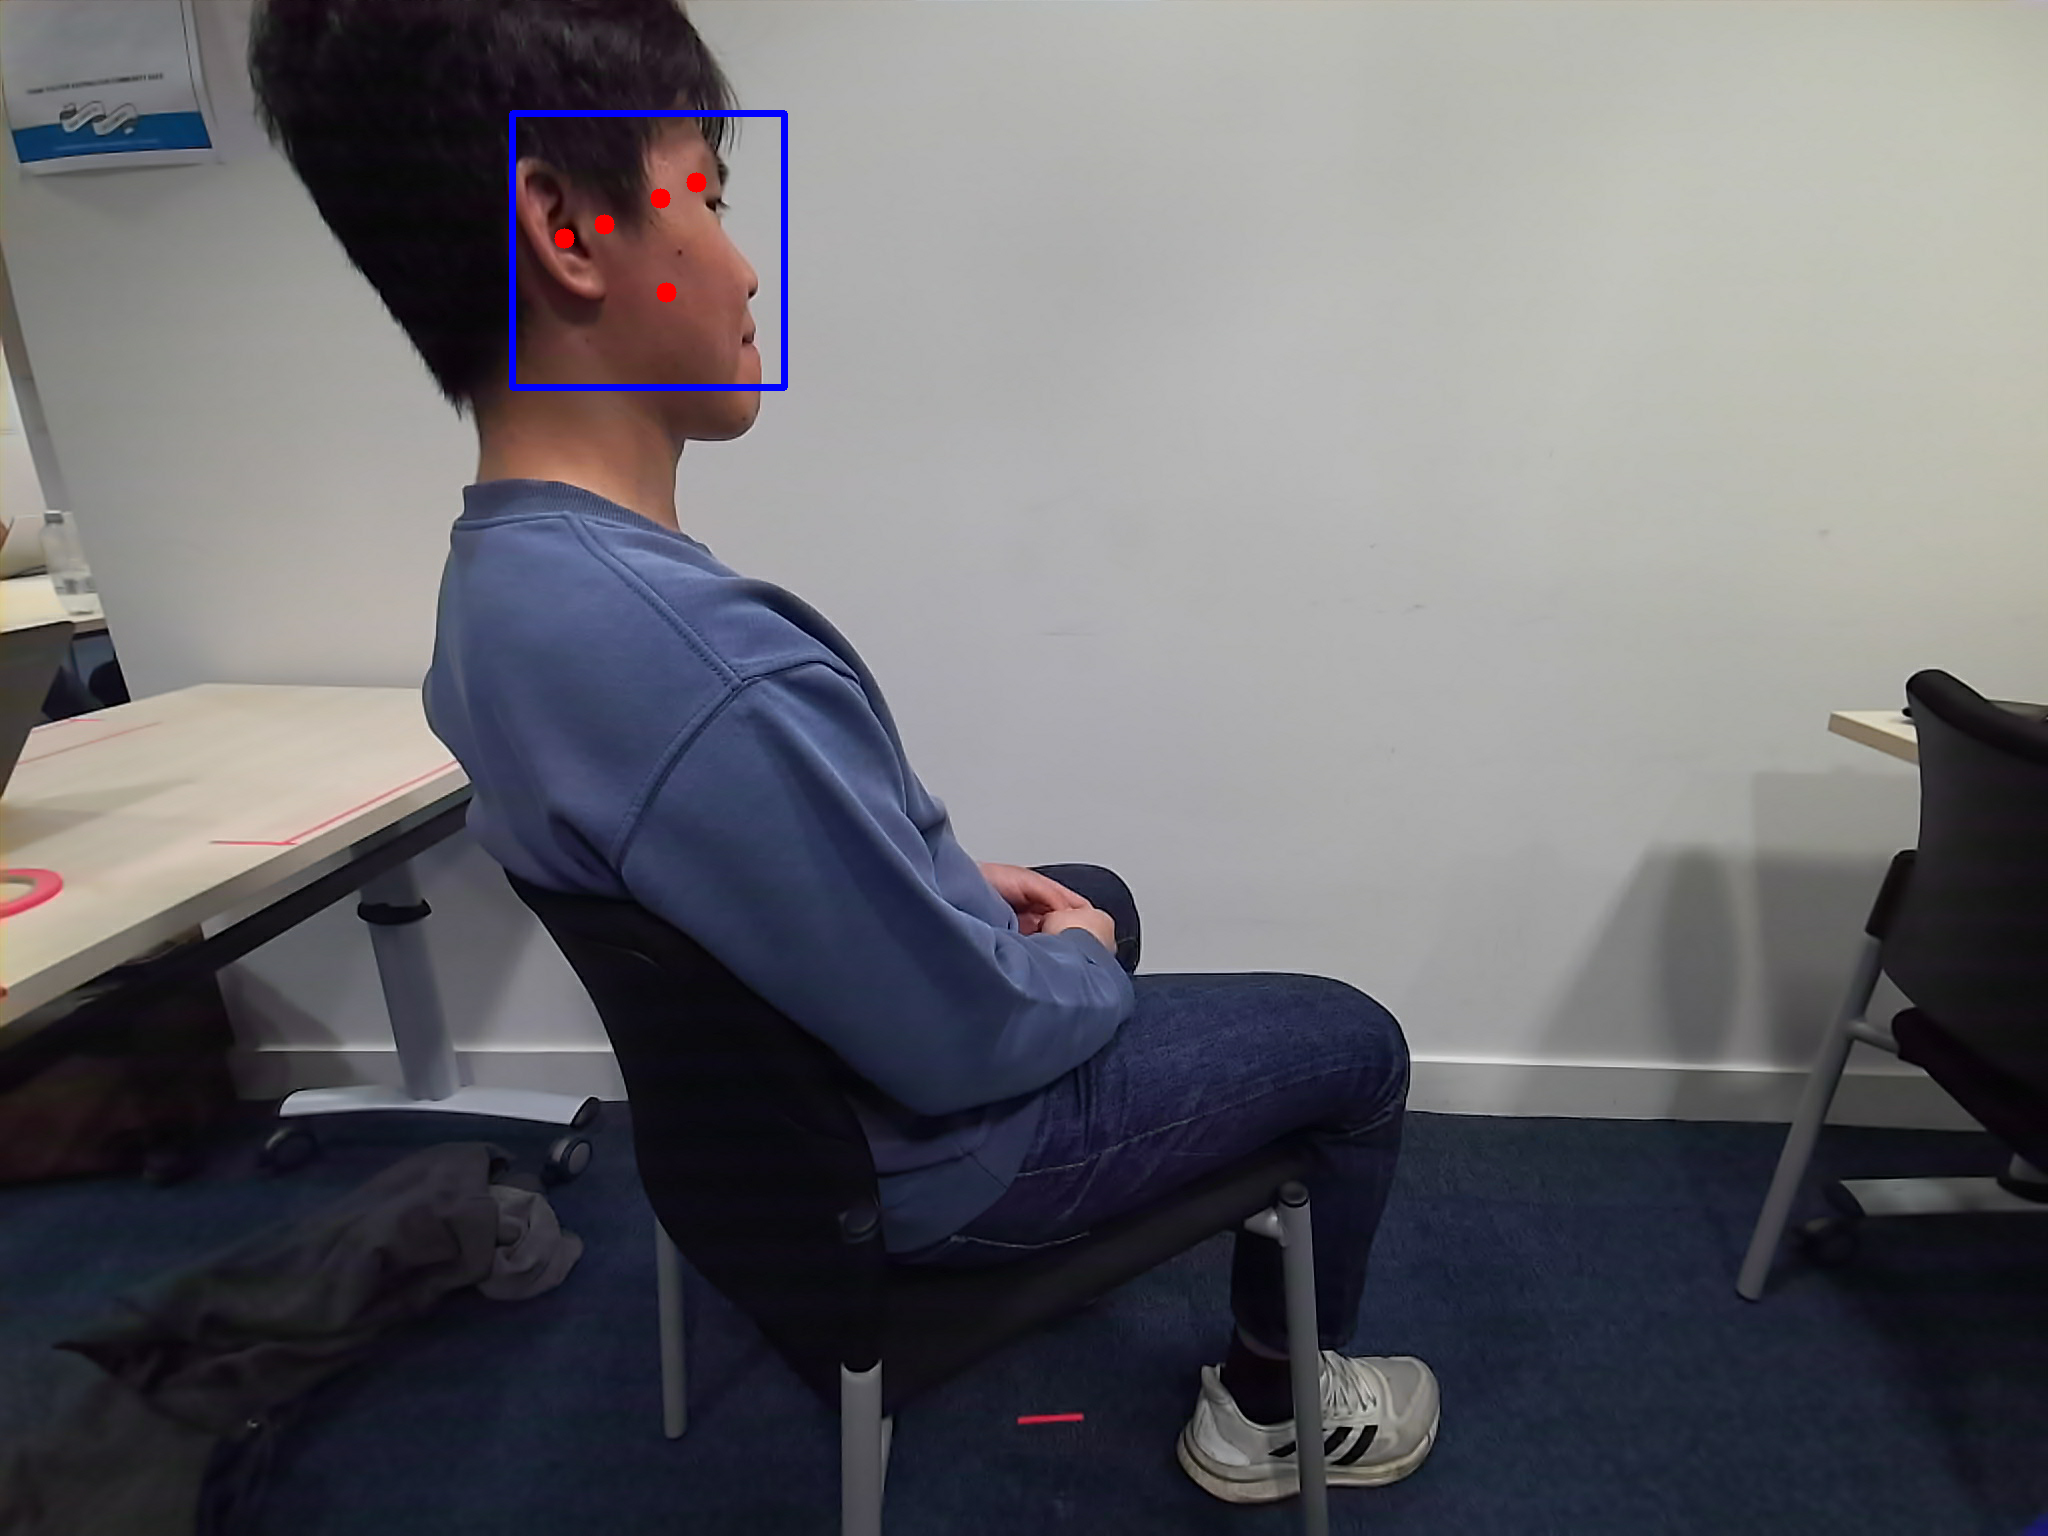
\includegraphics{./evaluation/figures/incorrectTrackedFace.png}
        }
    }
\end{invisBox}

As shown in Figure~\ref{fig:incorrect-head-track}, the face tracking model can still detect a face even when it is not visible, such as when detecting the side of the participant's head. The model tends to fail when only hair is visible. Testing on a bald participant could determine whether the system always detects a head regardless of rotation. While this might seem problematic, it is not, as the tracker and display are not visible to the user if their face is not visible. This also allows the system to approximate the position of the eyes, facilitating a smoother transition as the user turns their head back into view, minimizing the need for corrections and reducing noticeable adjustments for the user.

\subsubsection{Hand Tracking}

During the evaluation of our hand tracking model, we observed that it was significantly less reliable compared to our head tracking model, even when tested on the same images. Based on the metrics recorded during our user study, as illustrated in Fig~\ref{fig:failrate}, the hand tracking model failed for some users up to 10\% of the time, whereas the eye tracking model rarely experienced failures. When participants were surveyed about this during our user study they echoed our observations as can be seen in Fig~\ref{fig:reliable} with a noticeable drop in the rating of hand tracking reliability. This issue was particularly prominent when the model attempted to initially detect the hand. We found that the model was sensitive to specific conditions: it required a well-lit environment, a plain background, and the removal of extraneous objects from the scene. Users wearing t-shirts with intricate patterns experienced a notable decrease in tracking success. To address this, we provided a plain jumper for users to wear if we identified this as a potential problem. \\

We considered mitigating this issue by employing a segmentation model to separate the hand from the background before tracking. However, we did not have sufficient time to experiment with this solution, and we were concerned that it might significantly degrade the system's latency performance.

\begin{invisBox}
    \pictureBox[label={fig:failrate}]{Failure rates during user study}{
        \adjustbox{height=5cm, keepaspectratio}{
            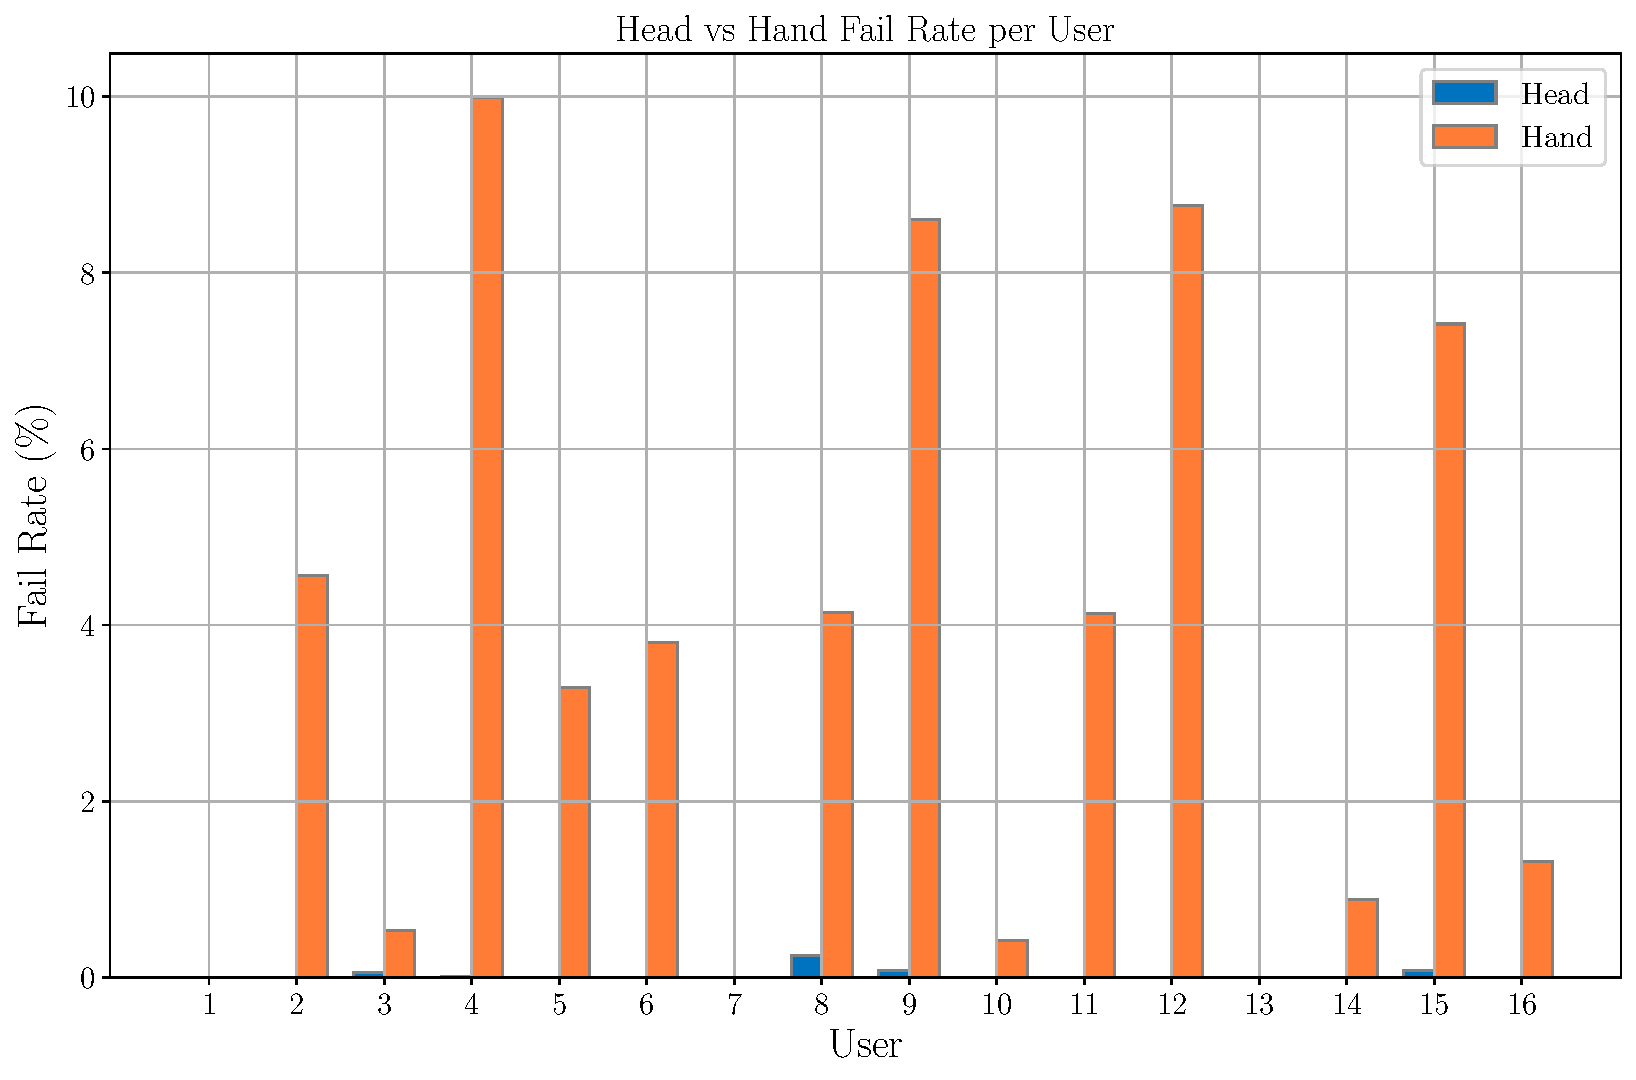
\includegraphics{./evaluation/figures/failrate.pdf}
        }
    }
    \hfill
    \pictureBox[label={fig:reliable}]{Accuracy and Reliability of Hand and Eye Tracking Survey}{
        \adjustbox{height=4.5cm, keepaspectratio}{
            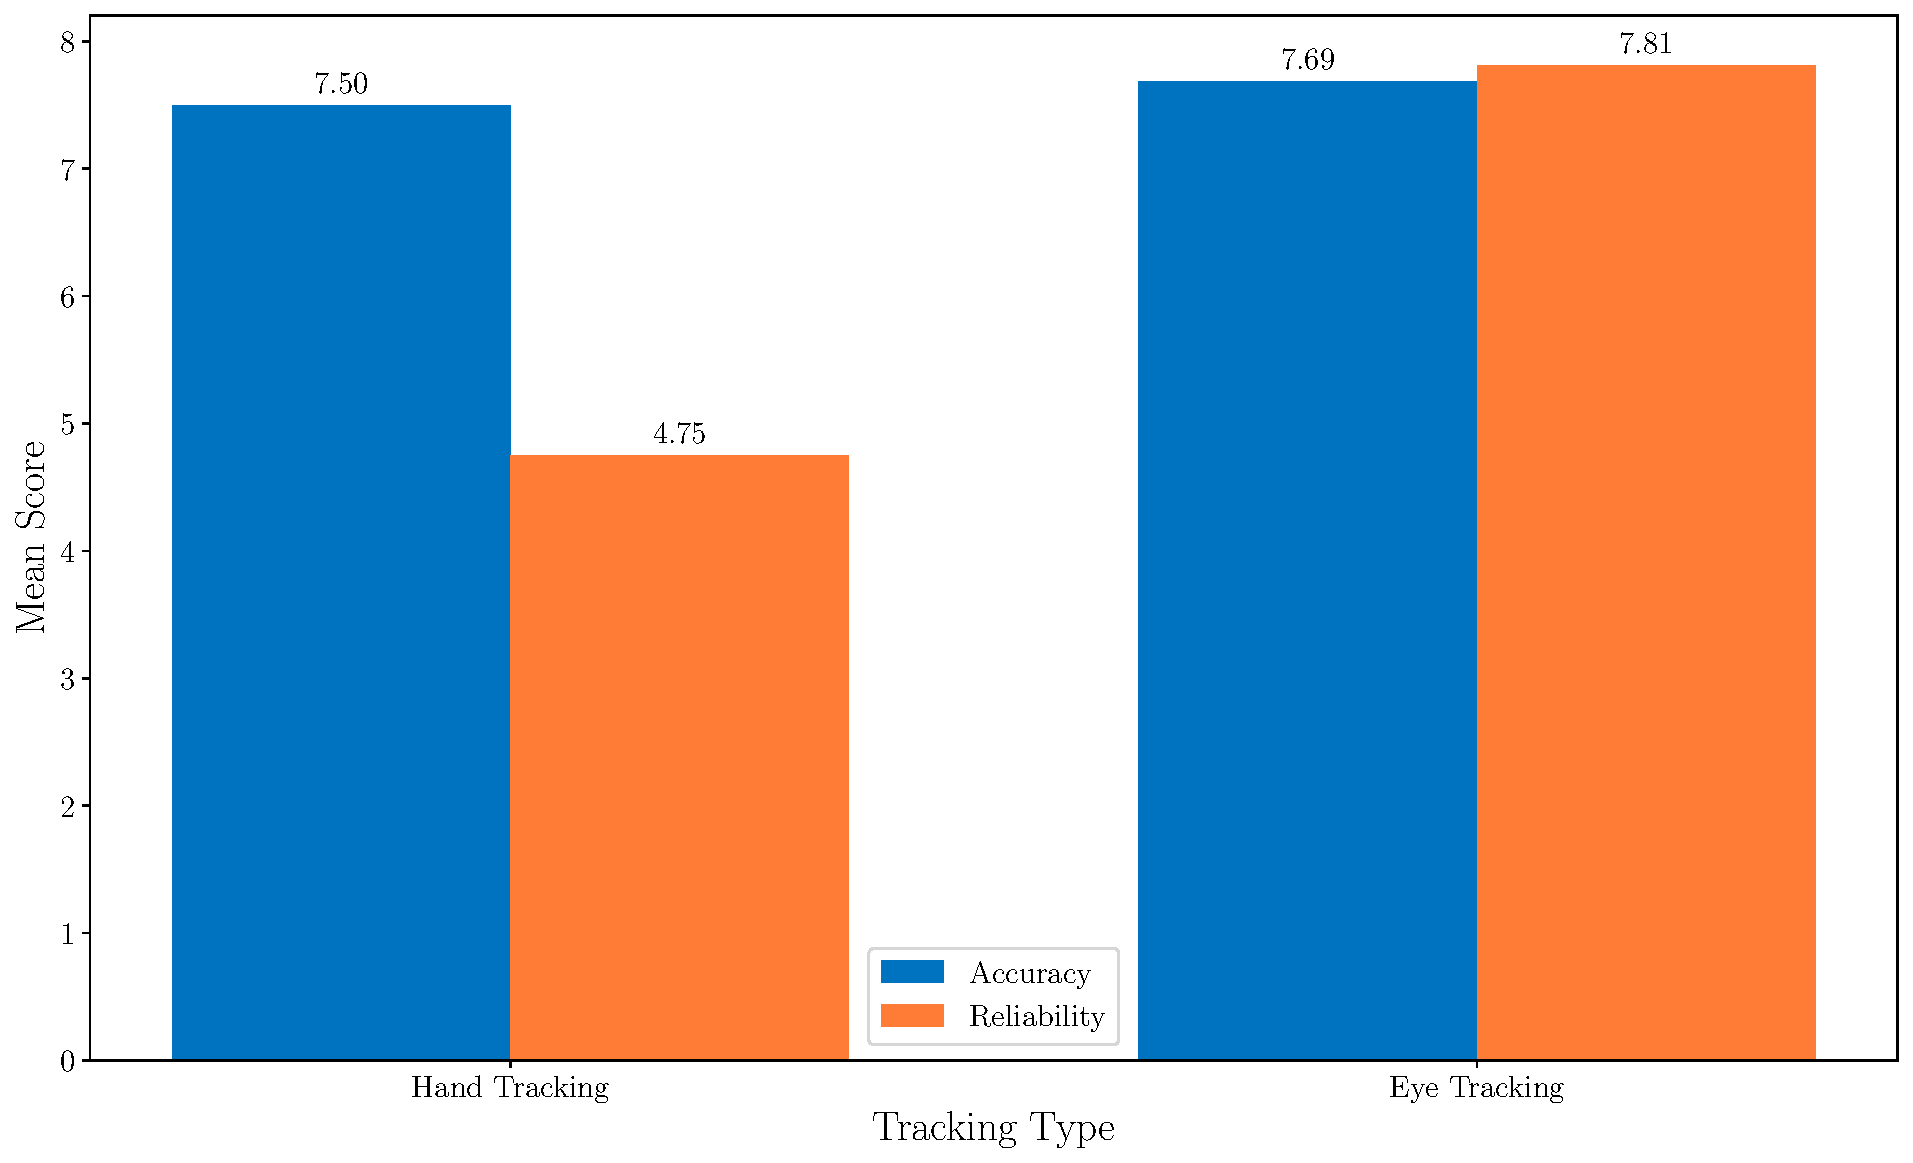
\includegraphics{./evaluation/figures/survery/reliable-accurate.pdf}
        }
    }
\end{invisBox}

A major challenge of using a depth sampling method is its inability to handle occlusion effectively. Although Mediapipe can predict the position of hand points even when they are not directly visible, our method struggles to sample their 3D positions accurately in such cases. This is problematic because the hand often occludes itself, as demonstrated in Fig~\ref{fig:occlusion}, where fingers are occluded by the palm, leading to erroneous depth sampling of the palm instead. Initially, we were concerned that this might also affect glasses wearers. However, we discovered that the depth sampling method, which uses infrared (IR) technology, was able to penetrate through glass.

\begin{figureBox}[label={fig:occlusion}, width=1.0\linewidth]{Occlusion in Sampling}
    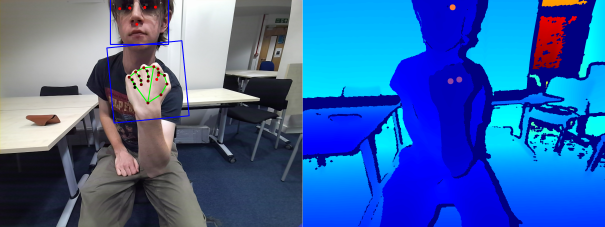
\includegraphics[width = 1.0\linewidth]{./evaluation/figures/occulusionsampling.png}
\end{figureBox}

There are methods to mitigate these issues, such as sampling from points that are not occluded and using the known depth of the hand to infer the depth of the occluded points. This is a complex problem, and we did not have sufficient time to develop a solution that was both accurate and fast. Additionally, we found that the relative depth values estimated by Mediapipe were not very accurate, complicating interaction. We believe that the most effective solution would be to switch to a point cloud-based tracking model \cite{sharp2015accurate}. Our solution was to switch to interaction using the middle and index fingers, the two fingers we found to be most reliable.

\subsection{Renderer}

In evaluating our rendering system, we focused primarily on the quality and accuracy of the images it produced.

\subsection{Quality}

To evaluate the quality of our rendering system, we rendered a variety of complex 3D objects, including a chess set, a Minecraft house, and a protein structure. The images produced by our system were of high quality, as shown in Figures~\ref{fig:chess}, \ref{fig:erato}, \ref{fig:house}, and \ref{fig:8qbk}. The system was able to render these objects with high fidelity, accurately representing their 3D structure. The images were sharp and detailed, with precise lighting and shading. The system effectively rendered complex objects with numerous details, such as the protein structure, without any noticeable loss of quality or drop in frame rate. The images produced by our system were comparable to those produced by professional rendering software, demonstrating the high quality of our system.

\begin{invisBox}  
	\pictureBox[label={fig:chess}]{Chess Set \cite{noauthor_chessset_nodate}}{
	  \adjustbox{height=5cm, keepaspectratio}{
		\includegraphics{./evaluation/figures/renderer/chess_croped.png}
	  }
	}
	\hfill
	\pictureBox[label={fig:erato}]{Erato \cite{McGuire2017Data}}{
	\adjustbox{height=5cm, keepaspectratio}{
	  \includegraphics{./evaluation/figures/renderer/erato_2_cropped.png}
	  }
	}
	\\[0.3cm]
	\pictureBox[label={fig:house}]{Minecraft House \cite{McGuire2017Data}}{
	  \adjustbox{height=5cm, keepaspectratio}{
		\includegraphics{./evaluation/figures/renderer/house_2_cropped.png}
	  }
	}
	\hfill
	\pictureBox[label={fig:8qbk}]{Retron-Eco1 filament with ADP-ribosylated Effector \cite{bank_rcsb_nodate}}{
	\adjustbox{height=5cm, keepaspectratio}{
	  \includegraphics{./evaluation/figures/renderer/8qbk_cropped.png}
	  }
	}
\end{invisBox}

We successfully loaded and rendered a 6 million triangle model of Rungholt, a medieval city that was destroyed by a storm surge in the 14th century and recreated in Minecraft, as shown in Figure~\ref{fig:rungholt}. The model was rendered with no frame rate issues, demonstrating the system's ability to handle large and complex models with ease.

\begin{figureBox}[label={fig:rungholt}, width=0.8\linewidth]{Rungholt \cite{McGuire2017Data}}
	\includegraphics[width = 1.0\linewidth]{./evaluation/figures/renderer/rungholt_cropped.png}
\end{figureBox}

\subsubsection{Accuracy}

To evaluate the accuracy of our rendering system, we aimed to determine how well it could recreate a real object in a virtual environment. We chose a cube as our test object due to its simplicity and ease of measurement. A physical cube was constructed using Lego, and a corresponding virtual cube was created in our simulator, both with the exact dimensions of 13.5 cm x 13.5 cm x 12 cm, as illustrated in Figure~\ref{fig:real-vs-rendered}.

\begin{figureBox}[label={fig:real-vs-rendered}, width=0.8\linewidth]{A real and rendered cube}
	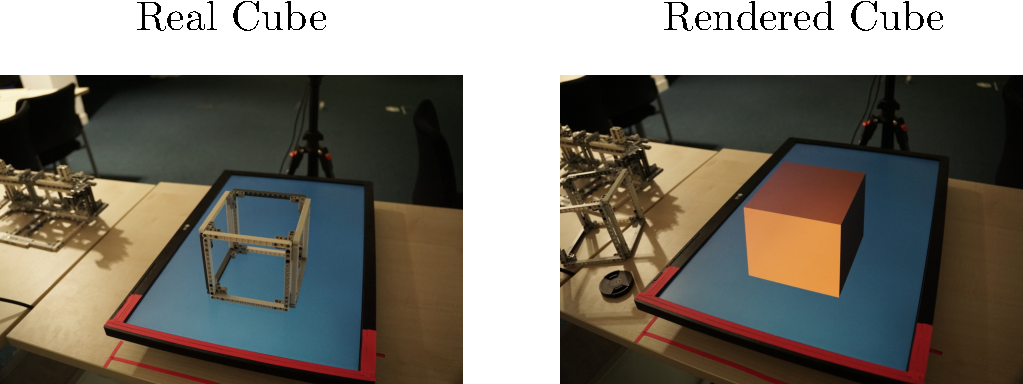
\includegraphics[width = 1.0\linewidth]{./evaluation/figures/real-vs-rendered.pdf}
\end{figureBox}

Due to the hollow nature of the physical cube, we were able to compare the two cubes effectively by superimposing them. We tested various perspectives and confirmed that the two cubes were indeed of the same size and shape, visually overlapping completely. Some example perspectives are presented in Figure~\ref{fig:super-imposed}. It is important to note that slight discrepancies in the images may occur, as the system was tracking the photographer's eye rather than the camera lens, which was positioned below and approximately 10 cm in front of the eye. Adjustments were made to account for this difference. This evaluation demonstrates that our rendering system is accurate and capable of recreating 3D objects from the real world with high precision.

\begin{figureBox}[label={fig:super-imposed}, width=0.8\linewidth]{Superimposed real and rendered cube}
	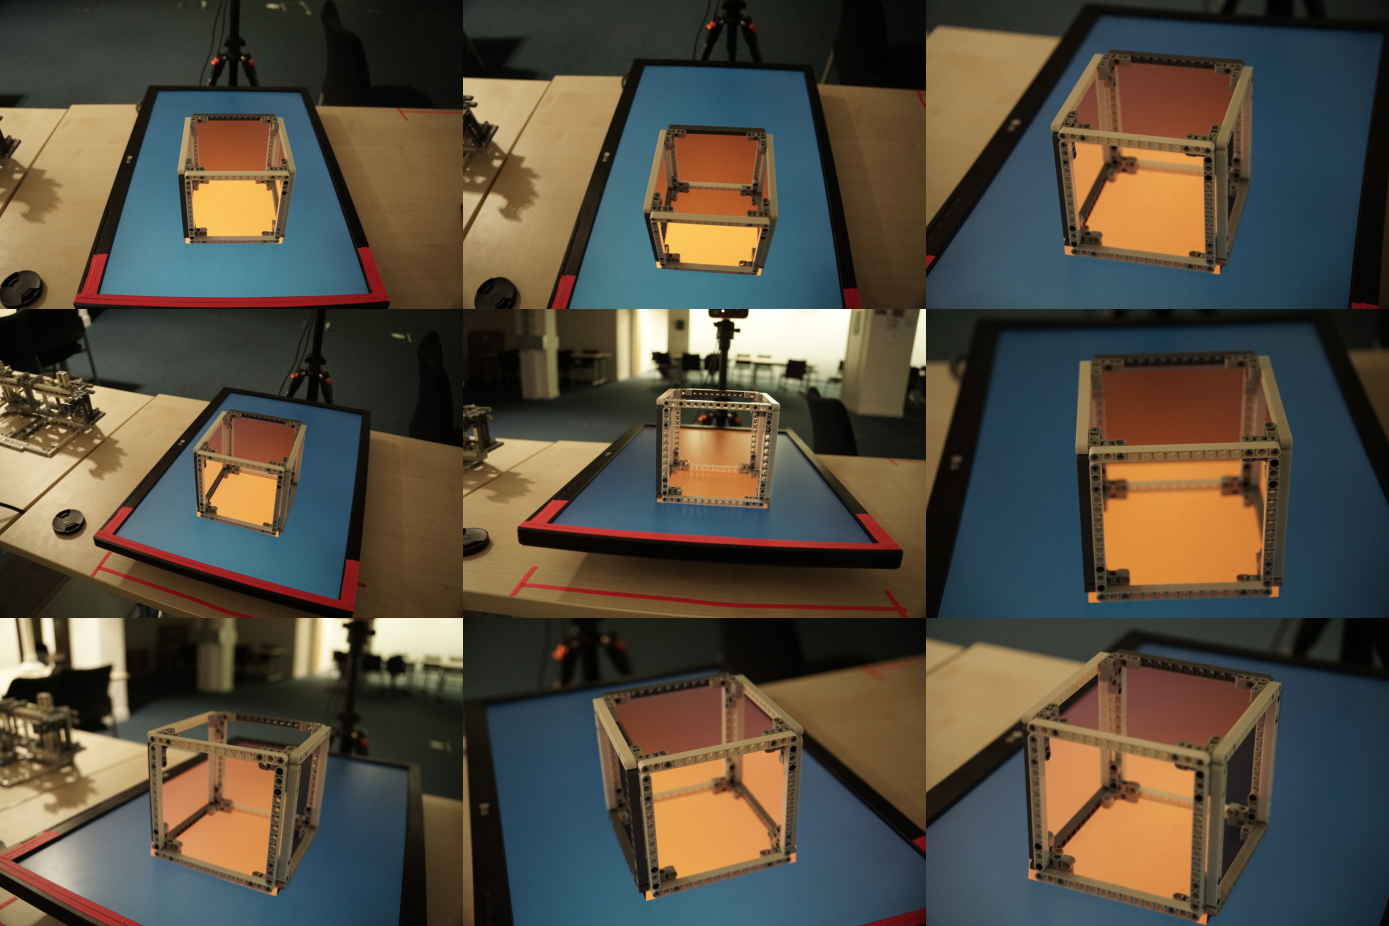
\includegraphics[width = 1.0\linewidth]{./evaluation/figures/super-imposed.pdf}
\end{figureBox}

It is worth noting that like all 3D rendering systems based on a 2D display medium, our system is subject to the limitations of dimensions of the screen. This means any object that extends beyond the screen will be clipped, and the user will not be able to see the entire object at once.

\subsection{Portability}
One of the significant advantages of this system is its reproducibility and ease of deployment. It can be set up on a fresh Linux machine from scratch with a single command. The system was developed on a Linux machine (NixOS) using an Intel i5-9600K CPU and an NVIDIA GeForce RTX 2070 Super GPU. For testing purposes, the system was also run on a different Linux machine (NixOS) equipped with an Intel i7-4770K CPU and an NVIDIA GeForce GTX 1080 GPU, as depicted in Fig.~\ref{fig:other-machine}. Remarkably, the system executed flawlessly on the first attempt on this different hardware configuration.

\begin{figureBox}[label={fig:other-machine}, width=0.7\linewidth]{Running on a different machine}
	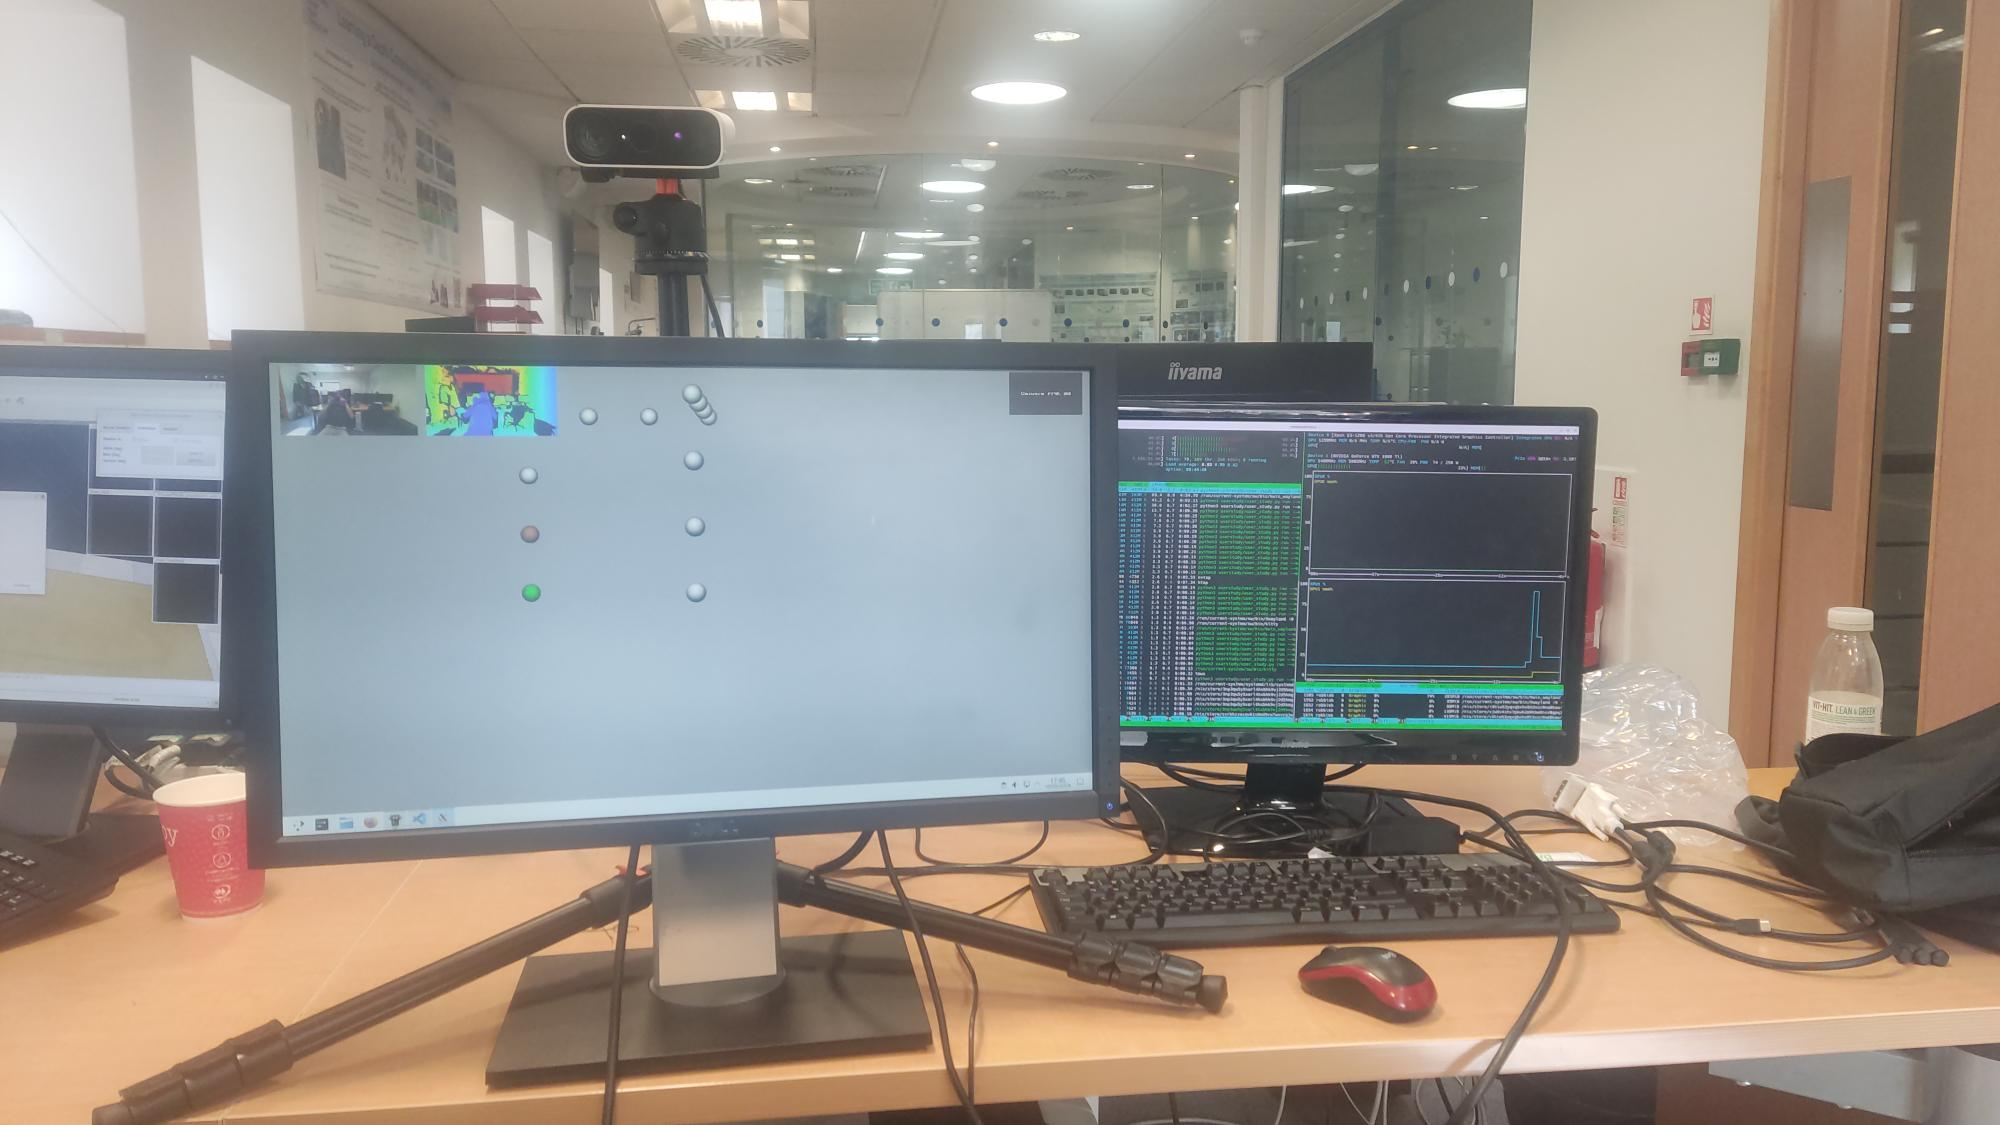
\includegraphics[width=1.0\linewidth]{./evaluation/figures/other-device.jpeg}
\end{figureBox}

We also tested the system on a Windows machine using Windows Subsystem for Linux 2 (WSL2). Although we successfully built the system, the OpenGL renderer did not function as expected. We did not have sufficient time to diagnose the issue thoroughly, but we suspect it is related to WSL GPU passthrough limitations. This issue is likely resolvable with additional troubleshooting. \\

Currently, the system only supports machines with Intel CPUs and NVIDIA GPUs. However, extending support to AMD CPUs and GPUs should be feasible with further development and fairly trivial modifications to the build system.

